\chapter{SPI sučelje i DMA prijenos}

SPI protokol se koristi za prijenos podataka između \textit{flash} memorije i mikrokontrolera, odnosno međuspremnika kamere. Kako bi se oslobodili resursi na mikrokontroleru, za prijenos podataka između kamere i \textit{flash} memorije se, u kombinaciji sa SPI protokolom, koristi i DMA prijenos. S obzirom na to da se koriste \textit{Low-Layer} biblioteke, potrebno je razumjeti način rada SPI i DMA periferija mikrokontrolera. U ovom poglavlju bit će opisan SPI protokol i DMA prijenos i bit će istaknute razlike i problemi kod prilagođavanja programske podrške za STM32L471VGT6 mikrokontroler.

\section{SPI protokol}

SPI je sinkrono serijsko komunikacijsko sučelje koje se koristi za komunikaciju na kratkim udaljenostima, pretežito u ugradbenim računalnim sustavima \cite{spi_wikipedia}. 

SPI uređaji komuniciraju u \textit{full-duplex} načinu rada koristeći \textit{master-slave} arhitekturu, obično sa jednim \textit{master} uređajem. \textit{Master} (upravljač) uređaj proizvodi okvir za čitanje i pisanje. Više \textit{slave} uređaja može biti spojeno na jedan upravljač tako da se aktivira određeni \textit{chip select} signal za pojedini uređaj.

\subsection{Opis sučelja}

SPI sabirnica se sastoji od četiri signala:
\begin{itemize}
	\item SCLK: Serijski takt (izvor je \textit{master} uređaj)
	\item MOSI: \textit{Master Output Slave Input} (izvor podataka iz \textit{master} uređaja)
	\item MISO: \textit{Master Input Slave Output} (izvor podataka iz \textit{slave} uređaja)
	\item CS/SS: \textit{Chip/Slave Select} (aktivan nisko, signal iz \textit{master} uređaja, označava da se prenose podaci)
\end{itemize}
MOSI na \textit{master} uređaju se spaja na MOSI na \textit{slave} uređaju, dok se MISO na \textit{master} uređaju se spaja na MISO na \textit{slave} uređaju. CS/SS se koristi za pokretanje komunikacije između \textit{slave} i \textit{master} uređaja. Za svaki \textit{slave} uređaj postoji zaseban CS/SS priključak na \textit{master} uređaju. Takav način spajanja se naziva neovisni \textit{slave} uređaj. Primjer spajanja tri \textit{slave} uređaja na jedan \textit{master} uređaj u konfiguraciji neovisnog \textit{slave} uređaja prikazan je na slici \ref{fig:spi_three_slaves}.
\begin{figure}[H]
	\centering
	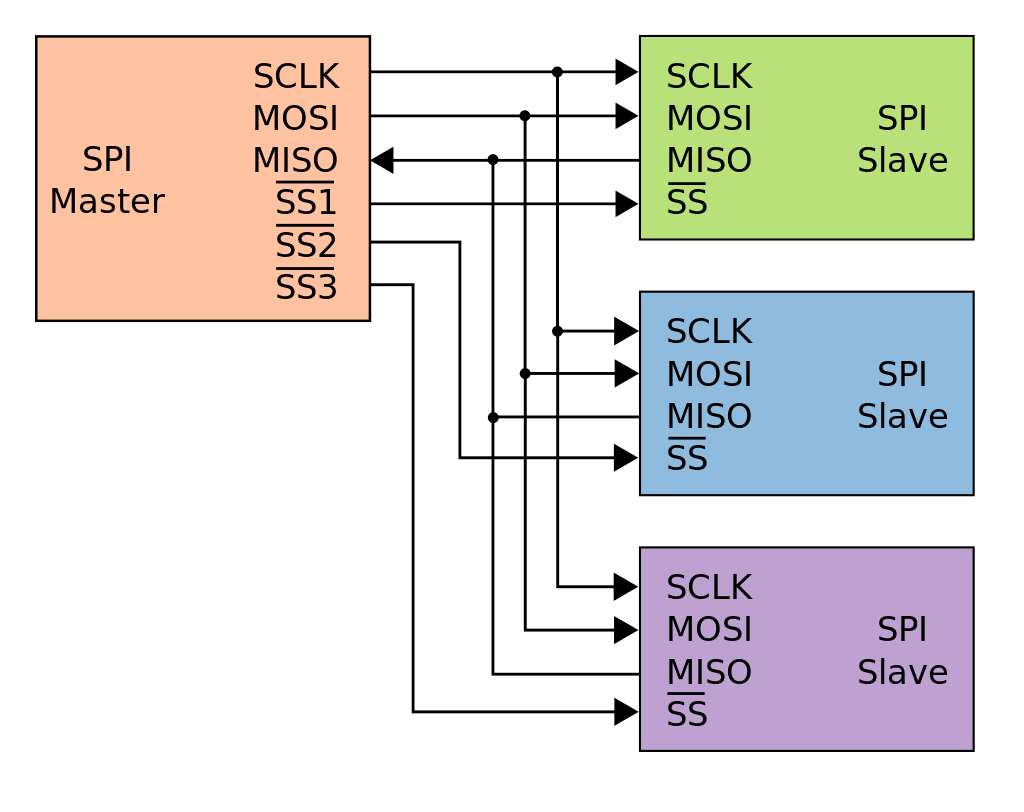
\includegraphics[height=7 cm]{SPI_three_slaves.svg.png}
	\caption{Spoj tri \textit{slave} uređaja na jedan \textit{master} uređaj u konfiguraciji neovisnog \textit{slave} uređaja. Vidljivo je da \textit{master} uređaj ima tri SS priključka, a svaki odgovara jednom \textit{slave} uređaju, dok se SCLK, MOSI i MISO linije međusobno dijele između \textit{slave} uređaja \cite{spi_wikipedia}}
	\label{fig:spi_three_slaves}
\end{figure}
Moguće je još spojiti uređaje u konfiguraciju ulančavanog \textit{slave} uređaja. U toj konfiguraciji \textit{slave} uređaji dijele isti CS/SS, a ulančavanjem preko MISO/MOSI linija podaci se prenose prema načelu posmačnog registra, koji je objašnjen u sljedećem potpoglavlju. Prikaz spajanja tri \textit{slave} uređaja se nalazi na slici \ref{fig:SPI_three_slaves_daisy_chained}.
\begin{figure}[H]
	\centering
	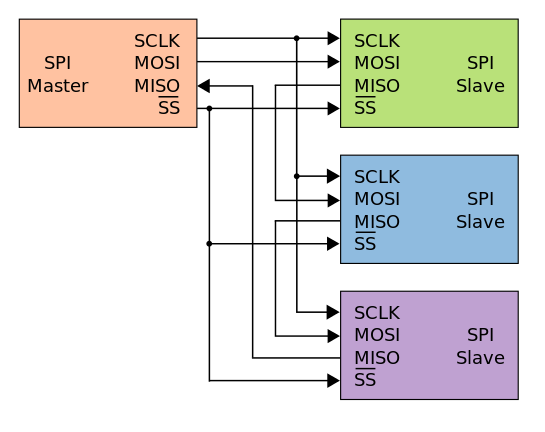
\includegraphics[height=7 cm]{SPI_three_slaves_daisy_chained.svg.png}
	\caption{Spoj tri \textit{slave} uređaja na jedan \textit{master} uređaj u konfiguraciji ulančavanog \textit{slave} uređaja \cite{spi_wikipedia}}
	\label{fig:SPI_three_slaves_daisy_chained}
\end{figure}

\subsection{Način rada}

SPI sabirnica radi s jednim \textit{master} uređajem i jednim ili više \textit{slave} uređaja. Ako se koristi jedan \textit{slave} uređaj, onda CS signal može biti postavljen u nisku logičku razinu, ako \textit{slave} uređaj to dopušta. Neki \textit{slave} uređaji zahtijevaju padajući brid CS signala kako bi započela komunikacija. Ako se koristi više \textit{slave} uređaja potreban je zaseban CS signal \textit{master} uređaja za svaki \textit{slave} uređaj.

\subsubsection{Prijenos podataka}

Za početak komunikacije \textit{master} uređaj konfigurira takt koristeći frekvenciju koju podržava \textit{slave} uređaj, obično do nekoliko MHz. \textit{Master} uređaj zatim odabire \textit{slave} uređaj postavljanjem CS linije u nisko logičko stanje. Ako je potreban period čekanja, npr. za AD (analogno-digitalnu) pretvorbu, \textit{master} uređaj mora pričekati minimalno taj period vremena prije puštanja takta.

Tijekom svakog perioda takta obavlja se prijenos podataka u \textit{full-duplex} načinu rada. To znači da \textit{master} uređaj pošalje jedan bit na MOSI liniju, koji \textit{slave} uređaj pročita, dok u isto vrijeme \textit{slave} uređaj šalje jedan bit na MISO liniju, koji \textit{master} uređaj pročita. Takva sekvenca se održava čak i kada se izvodi jednosmjerni prijenos podataka.

Prijenosi podataka uključuju dva posmačna registra zadane veličine, npr. 8 bitova, jedan u \textit{master} i drugi u \textit{slave} uređaju. Registri su spojeni u topologiji virtualnog prstena (slika \ref{fig:spi_circular_transfer}).
\begin{figure}[H]
	\centering
	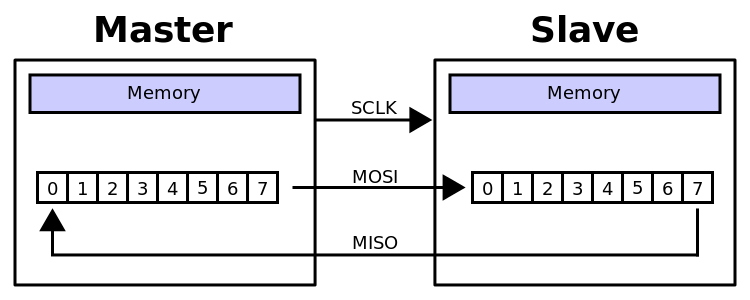
\includegraphics[width=\textwidth]{SPI_8-bit_circular_transfer.svg.png}
	\caption{Tipičan spoj dvaju posmačna registra koji formiraju kružni međuspremnik \cite{spi_wikipedia}}
	\label{fig:spi_circular_transfer}
\end{figure}
Podaci se obično pomiču tako da se prvo pomakne najznačajniji bit. Na brid takta, \textit{master} i \textit{slave} uređaj pomaknu bit i pošalju ga na prijenosnu liniju. Na sljedeći brid takta, na svakom prijamniku bit se uzorkuje s prijenosne linije i postavlja se kao novi najmanje značajni bit u posmačnom registru. \textit{Master} i \textit{slave} uređaji u potpunosti razmjene podatke u registrima nakon što se svi bitovi u registrima prebace. Ako je potrebno razmijeniti još podataka, posmačni registri se ponovno napune te se postupak ponavlja, a prijenos se može obavljati za bilo koji broj perioda takta. Kada je prijenos dovršen, \textit{master} uređaj prestaje davati takt i obično isključi CS signal, odnosno postavi ga na visoku razinu.

Prijenos se obično obavlja u riječima širine 8 bitova, no moguća je i širina riječi od 12 bita, ili čak 12 bitova, koji se koristi za digitalno-analogne i analogno-digitalne pretvornike.

\subsubsection{Polaritet takta i faza}

Osim što mora podesiti frekvenciju takta, \textit{master} uređaj mora isto tako podesiti polaritet takta (CPOL, engl. \textit{Clock Polarity}) i fazu (CPHA, engl. \textit{Clock Phase}) ovisno o podacima. Vremenski dijagram je prikazan na slici \ref{fig:spi_timing_diagram}.
\begin{figure}[H]
	\centering
	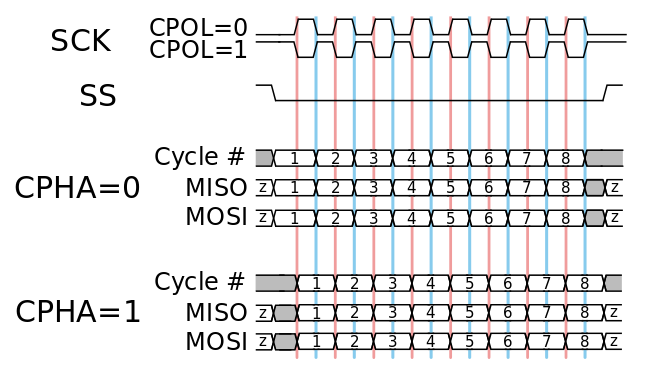
\includegraphics[height=7 cm]{SPI_timing_diagram2.svg.png}
	\caption{Vremenski dijagram koji pokazuje polaritet takta i fazu. Crvene linije označuju vodeće bridove, a plave linije označavaju prateće bridove.}
	\label{fig:spi_timing_diagram}
\end{figure}
CPOL određuje polaritet kanala. Polaritet može biti invertiran jednostavnim inverterom.
\begin{itemize}
	\item Ako je CPOL = 0, onda takt miruje u niskom logičkom stanju, a svaki period se sastoji od impulsa visokog logičkog stanja. To znači da je vodeći brid rastući brid, a prateći brid padajući brid.
	\item Ako je CPOL = 1, onda takt miruje u visokom logičkom stanju, a svaki period se sastoji od impulsa niskog logičkog stanja. To znači da je vodeći brid padajući brid, a prateći brid rastući brid.
\end{itemize}
CPHA određuje fazu podatkovnih bitova u odnosu na takt.
\begin{itemize}
	\item Ako je CPHA = 0, "izlazna" strana mijenja podatak na prateći brid prethodnog perioda takta, dok "ulazna" strana prihvaća podatak na (ili ubrzo nakon) vodeći brid perioda takta. Izlazna strana zadržava valjani podatak sve do pojave pratećeg brida trenutnog perioda takta.
	\item Ako je CPHA = 1, "izlazna" strana mijenja podatak na vodeći brid trenutnog perioda takta, dok "ulazna" strana prihvaća podatak na (ili ubrzo nakon) pratećeg brida perioda takta. Izlazna strana zadržava valjani podatak do pojave vodećeg brida sljedećeg perioda takta. Na zadnji period, \textit{slave} uređaj zadržava valjani podatak na MISO liniji sve dok \textit{slave} uređaj ne bude deselektiran.
\end{itemize}
MOSI i MISO signali su obično stabilni za vrijeme pola perioda takta, sve do sljedeće promjene takta. SPI \textit{master} i \textit{slave} uređaji mogu uzorkovati podatke u bilo kojem vremenu unutar te polovice periode takta.

Kombinacije različitih konfiguracija CPOL i CPHA bitova predstavljaju načine rada. Konvnecija je da CPOL predstavlja viši bit, dok CPHA predstavlja niži bit. Načini rada kod ARM-ovih mikrokontrolera su prikazani u tablici \ref{Tab:spi_modes}
\begin{center}
	\begin{table}[H]
		\centering
		\begin{tabular}{| c | c | c |}
			\hline
			SPI način rada & CPOL & CPHA \\
			\hline
			0 & 0 & 0 \\
			\hline
			1 & 0 & 1 \\
			\hline
			2 & 1 & 0 \\
			\hline
			3 & 1 & 1 \\
			\hline
		\end{tabular}
		\caption{SPI načini rada kod ARM-ovih mikrokontrolera \cite{spi_wikipedia}}
		\label{Tab:spi_modes}
	\end{table}
\end{center}

\section{Prijenos programske podrške sa STM32F407VGT6 mirokontrolera na STM32L471VGT6 mikrokontroler}

Što se tiče programske podrške za SPI komunikaciju između mikrokontrolera, \textit{flash} memorije i kamere, nije došlo do nikakvih poteškoća kod prijenosa programske podrške s prethodno korištenog mikrokontrolera na trenutni. Razlike između SPI periferijskih sklopova STM32F407VGT6 i STM32L471VGT6 mikrokontrolera postoje, međutim, s obzirom na način koji se SPI protokol koristi u ovom projektu, te razlike su zanemarive i može se reći da SPI komunikacija na trenuračno korištenom mikrokontroleru funkcionira na isti način kao i na prethodno korištenom mikrokontroleru.

Došlo je, međutim, do poteškoća kod prijenosa programske podrške za DMA prijenos, koje će biti objašnjene u sljedećem poglavlju.

\section{DMA prijenos}

DMA se koristi kako bi se omogućio prijenos podataka visokih brzina između periferijskih sklopova i memorije ili između jedne memorije i druge memorije \cite{f407_manual}. Podatci se brzo mogu prenijeti bez posredovanja procesora. Na taj se način oslobađaju resursi procesora kako bi se mogle druge operacije za vrijeme prijenosa.

U ovom projektu DMA prijenos se koristi između međuspremnika kamere i radne memorije mikrokontrolera.

\subsection{Razlike DMA periferije na STM32F407VGT6 i STM32L471VGT6 mikrokontrolerima}

STM32F407VGT6 mikrokontroler ima dva DMA kontrolera. Blok dijagram jednog DMA kontrolera je prikazan na slici \ref{fig:f407_dma_block_diagram}.

\begin{figure}[H]
	\centering
	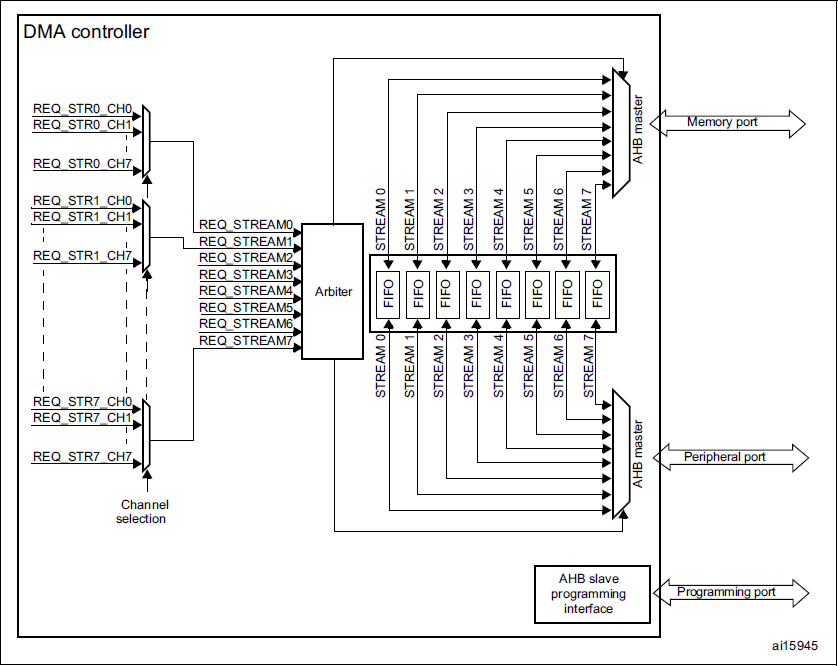
\includegraphics[height=10 cm]{f407_dma_block_diagram.png}
	\caption{Blok dijagram DMA kontrolera na STM32F407VGT6 mikrokontroleru \cite{f407_manual}}
	\label{fig:f407_dma_block_diagram}
\end{figure}

DMA kontroler obavlja izravan prijenos memorije; kao AHB \textit{master}, može u bilo kojem trenutku preuzeti kontrolu nad AHB sabirnicom i pokrenuti AHB transakcije. DMA kontroler može pokrenuti sljedeće transakcije:
\begin{itemize}
	\item prijenos sa periferije na memoriju,
	\item prijenos sa memorije na periferiju,
	\item prijenos sa memorije na memoriju.
\end{itemize}
S obzirom na to da se u ovom radu koriste prijenosi s periferije na memoriju i obrnuto, u daljnjem tekstu će se podrazumijevati samo ti slučajevi.

DMA periferija ima dvije AHB \textit{master} sabirnice, jedna se koristi za pristup memoriji, a druga za pristup periferijama. AHB \textit{slave} vrata se koriste za programiranje DMA kontrolera.

Pojedini kontroler ima 8 tokova (engl. \textit{stream}), te za svaki tok postoji 8 kanala (engl. \textit{channel}). Svaki tok je spojen na određeni sklopovski DMA kanal. Tokovi i kanali služe kako bi se ostvarila veza između ostalih periferija i DMA mikorkontrolera, tako da periferije mogu slati zahtjev za DMA prijenos. %Broj podataka koji se trebaju prenijeti (do 65535) je programabilan i povezan je sa širinom izvora periferije koja zahtijeva DMA prijenos. Registar koji sadržava broj podataka koji se trebaju prenijeti se dekrementira nakon svake transakcije.

Svaki DMA prijenos se sastoji od tri operacije:
\begin{itemize}
	\item učitavanje sa periferijskog podatkovnog registra ili lokacije u memoriji, čije su adrese zapisane u DMA\_SxPAR ili DMA\_SxM0AR registru
	\item spremanje podataka na periferijski podatkovni registar ili lokaciju u memoriji, čije su adrese zapisane u DMA\_SxPAR ili DMA\_SxM0AR registru
	\item naknadno dekrementiranje DMA\_SxNDTR registra, koji sadržava broj podataka koji se još trebaju prenjeti
\end{itemize}
Spomenuti registri su prikazani u tablici \ref{Tab:f407_dma_register_map_1}. Kada periferija želi pristupiti DMA kontroleru, periferijski sklop šalje zahtjev DMA kontroleru. DMA kontroler poslužuje zahtjev ovisno o prioritetima kanala. Čim DMA kontroler pristupi periferiji, DMA kontroler periferiji šalje signal potvrde. Periferni uređaj ukida svoj zahtjev čim dobije potvrdni signal iz DMA kontrolera. Nakon što periferna jedinica ukine zahtjev, DMA kontroler ukida signal potvrde. Ako ima više zahtjeva, periferna jedinica može pokrenuti sljedeću transakciju.

\begin{table}[H]
	\resizebox{\textwidth}{!}{%
	\begin{tabular}{|c|c|l|l|l|l|l|l|l|l|l|l|l|l|l|l|l|l|l|l|l|l|l|l|l|l|l|l|l|l|l|l|l|}
		\hline
		\textbf{\begin{tabular}[c]{@{}c@{}}Register\\ name\end{tabular}} & \rotbf{31} & \rotbf{30} & \rotbf{29} & \rotbf{28} & \rotbf{27} & \rotbf{26} & \rotbf{25} & \rotbf{24} & \rotbf{23} & \rotbf{22} & \rotbf{21} & \rotbf{20} & \rotbf{19} & \rotbf{18} & \rotbf{17} & \rotbf{16} & \rotbf{15} & \rotbf{14} & \rotbf{13} & \rotbf{12} & \rotbf{11} & \rotbf{10} & \rotbf{9} & \rotbf{8} & \rotbf{7} & \rotbf{6} & \rotbf{5} & \rotbf{4} & \rotbf{3} & \rotbf{2} & \rotbf{1} & \rotbf{0} \\
		\hline
		DMA\_SxPAR & \multicolumn{32}{c|}{PA[31:0]} \\
		\hline
		Reset value & 0 & 0 & 0 & 0 & 0 & 0 & 0 & 0 & 0 & 0 & 0 & 0 & 0 & 0 & 0 & 0 & 0 & 0 & 0 & 0 & 0 & 0 & 0 & 0 & 0 & 0 & 0 & 0 & 0 & 0 & 0 & 0 \\
		\hline
		DMA\_M0AR & \multicolumn{32}{c|}{M0A[31:0]} \\
		\hline
		Reset value & 0 & 0 & 0 & 0 & 0 & 0 & 0 & 0 & 0 & 0 & 0 & 0 & 0 & 0 & 0 & 0 & 0 & 0 & 0 & 0 & 0 & 0 & 0 & 0 & 0 & 0 & 0 & 0 & 0 & 0 & 0 & 0 \\
		\hline
		DMA\_SxNDTR & \multicolumn{16}{c|}{Res.} & \multicolumn{16}{c|}{NDT[15:0]}\\
		\hline
		Reset value & & & & & & & & & & & & & & & & & 0 & 0 & 0 & 0 & 0 & 0 & 0 & 0 & 0 & 0 & 0 & 0 & 0 & 0 & 0 & 0 \\
		\hline
	\end{tabular}%
	}
	\caption{Registri DMA\_SxPAR, DMA\_SxM0AR i DMA\_SxNDTR kod STM32F407VGT6 mikrokontrolera. \textit{x} označava broj toka \cite{f407_manual}}
	\label{Tab:f407_dma_register_map_1}
\end{table}

Svaki tok je povezan sa DMA zahtjevom, koji može biti odabran između 8 mogućih kanalnih zahtjeva. Odabir kanala određuju bitovi CHSEL[2:0] u DMA\_SxCR registru (tablica \ref{Tab:f407_dma_register_map_2}). Odabir kanala prikazan je na slici \ref{fig:f407_dma_channel_selection}.
\begin{table}[H]
	\resizebox{\textwidth}{!}{%
	\begin{tabular}{|c|c|l|l|l|l|l|l|l|l|l|l|l|l|l|l|l|l|l|l|l|l|l|l|l|l|l|l|l|l|l|l|l|}
		\hline
		\textbf{\begin{tabular}[c]{@{}c@{}}Register\\ name\end{tabular}} & \rotbf{31} & \rotbf{30} & \rotbf{29} & \rotbf{28} & \rotbf{27} & \rotbf{26} & \rotbf{25} & \rotbf{24} & \rotbf{23} & \rotbf{22} & \rotbf{21} & \rotbf{20} & \rotbf{19} & \rotbf{18} & \rotbf{17} & \rotbf{16} & \rotbf{15} & \rotbf{14} & \rotbf{13} & \rotbf{12} & \rotbf{11} & \rotbf{10} & \rotbf{9} & \rotbf{8} & \rotbf{7} & \rotbf{6} & \rotbf{5} & \rotbf{4} & \rotbf{3} & \rotbf{2} & \rotbf{1} & \rotbf{0} \\
		\hline
		DMA\_SxPAR & \multicolumn{4}{c|}{Res.} & \multicolumn{3}{c|}{\rot{CHSEL[2:0]}} & \multicolumn{2}{c|}{\rot{MBURST[1:0]}} & \multicolumn{2}{c|}{\rot{PBURST[1:0]}} & \rot{Res.} & \rot{CT} & \rot{DBM} & \multicolumn{2}{c|}{\rot{PL[1:0]}} & \rot{PINCOS} & \multicolumn{2}{c|}{\rot{MSIZE[1:0]}} & \multicolumn{2}{c|}{\rot{PSIZE[1:0]}} & \rot{MINC} & \rot{PINC} & \rot{CIRC} & \multicolumn{2}{c|}{\rot{DIR[1:0]}} & \rot{PFCTRL} & \rot{TCIE} & \rot{HTIE} & \rot{TEIE} & \rot{DMEIE} & \rot{EN} \\
		\hline
		Reset value & & & & & 0 & 0 & 0 & 0 & 0 & 0 & 0 & & 0 & 0 & 0 & 0 & 0 & 0 & 0 & 0 & 0 & 0 & 0 & 0 & 0 & 0 & 0 & 0 & 0 & 0 & 0 & 0 \\
		\hline
	\end{tabular}%
	}
	\caption{Registar DMA\_SxCR kod STM32F407VGT6 mikrokontrolera \citep{f407_manual}}
	\label{Tab:f407_dma_register_map_2}
\end{table} 
\begin{figure}[H]
	\centering
	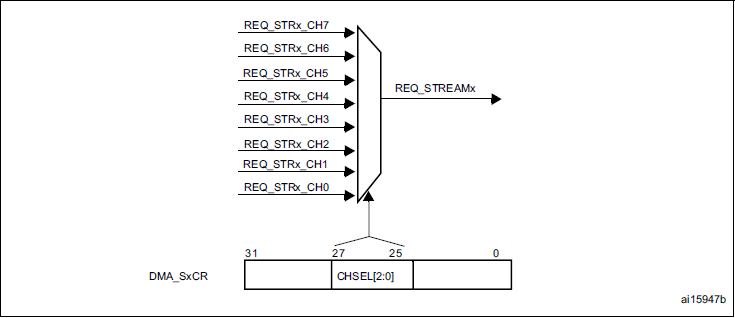
\includegraphics[width=\textwidth]{f407_dma_channel_selection.png}
	\caption{Odabir kanala \citep{f407_manual}}
	\label{fig:f407_dma_channel_selection}
\end{figure}
Proučavanjem dokumentacije mikrokontrolera, zaključeno je da kako bi se koristio SPI protokol s DMA prijenosom mora se koristiti kanal 0 i tokovi 3 (SPI2\_RX) i 4 (SPI2\_TX) \cite[str. 307]{f407_manual}. Odabrani tokovi se koriste zato što je kamera spojena na SPI2 periferiju mikrokontrolera.

Blok dijagram DMA periferije na STM32L471VGT6 mikrokontroleru je prikazan na slici \ref{fig:l471_dma_block_diagram}. Vidljivo je da oba mikrokontrolera sadržavaju dvije DMA periferije. Za razliku od SMT32F407VGT6 mikrokontrolera, trenutačni mikrokontroler, STM32L471VGT6, nema dvije AHB \textit{master} sabirnice, već samo jednu AHB \textit{master} sabirnicu.

\begin{figure}[H]
	\centering
	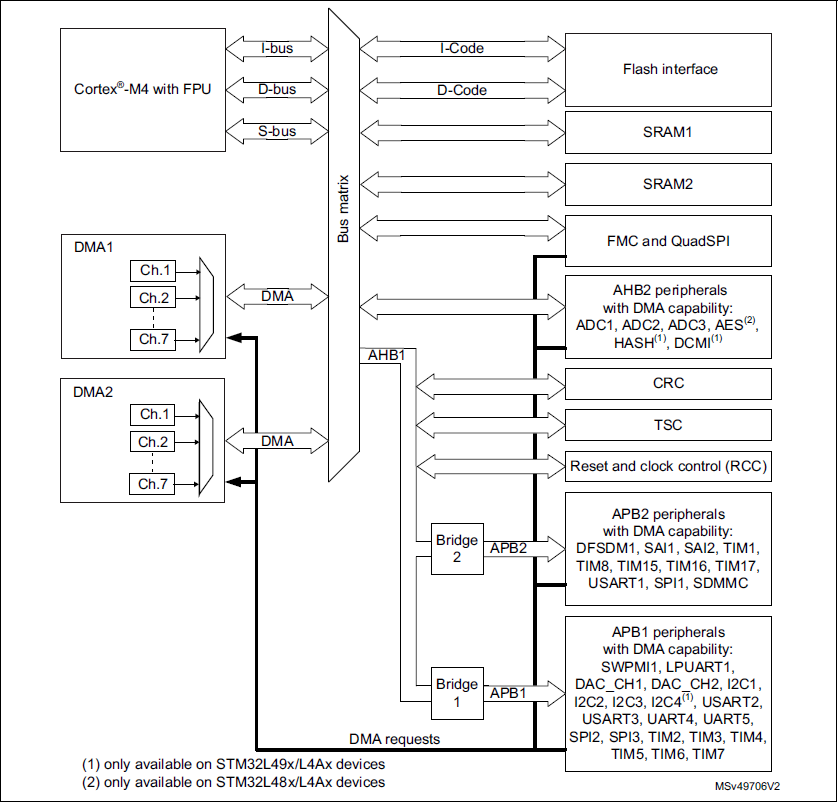
\includegraphics[height=10 cm]{l471_dma_block_diagram.png}
	\caption{Blok dijagram DMA periferije na STM32L471VGT6 mikrokontroleru \cite{l471_manual}}
	\label{fig:l471_dma_block_diagram}
\end{figure}

STM32L471VGT6 nema tokove kao vezu za zahtjevom prekida, već ima samo kanale, te se stoga veza između ostalih periferija i DMA kontrolera ostvaruje na drugačiji način, prikazan na slici \ref{fig:l471_dma_request_mapping}. Iz slike je vidljivo da se na ovom mikrokontroleru trebaju koristiti kanali 4 (SPI2\_RX) i 5 (SPI2\_TX).

\begin{figure}[H]
	\centering
	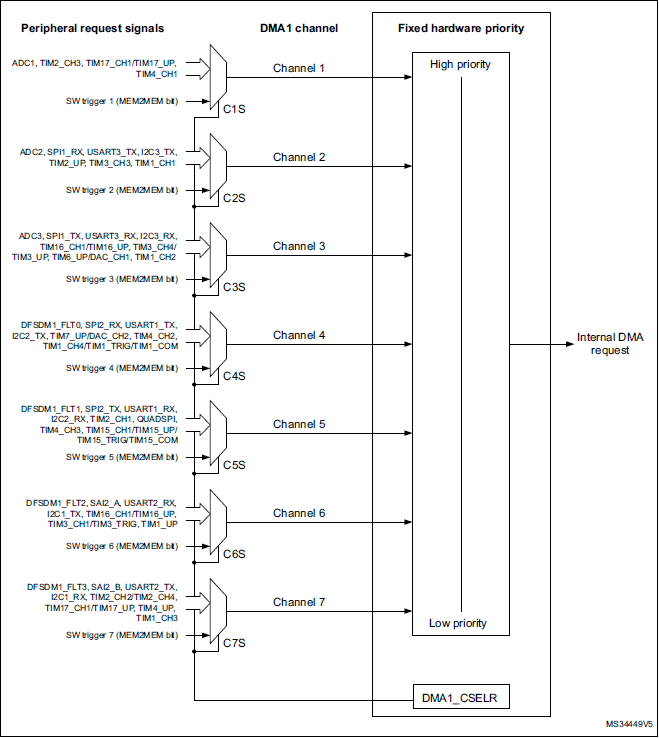
\includegraphics[width=10 cm]{l471_dma_request_mapping.png}
	\caption{Mapiranje zahtjeva za DMA1 kontroler kod STM32L471VGT6 mikrokontrolera \cite[str. 338]{l471_manual}}
	\label{fig:l471_dma_request_mapping}
\end{figure}

Još jedna razlika između DMA periferija dvaju mikrokontrolera se krije u prekidima koje DMA kontrolera i zastavicama za prekide. STM32F407VGT6 ima 5 različitih prekida: završetak prijenosa (TC, engl. \textit{Transfer Complete}), obavljena polovica prijenosa (HT, engl. \textit{Half Transfer}), greška u prijenosu (TE, engl. \textit{Transfer Error}), FIFO greška (FE, engl. \textit{FIFO Error}) i greška u direktnom načinu rada (DME, engl. \textit{Direct Mode Error}). STM32L471VGT6 ima 3 različita prekida: završetak prijenosa završetak prijenosa (TC), obavljena polovica prijenosa (HT), greška u prijenosu (TE). Kod STM32L471VGT6 postoji još globalni prekid (GI, engl. \textit{Global Interrupt}) koji se aktivira u svim slučajevima. Ako se, na primjer, želi DMA kontroler namjestiti da zahtijeva prekid kod završetka prijenosa, polovice prijenos i kod greške u prijenosu, to se može podesiti jednostavno aktiviranjem globalnih prekida. S obzirom na to STM32F407VGT6 sadržava više vrsta prekida, on sadržava i 2 prekidna registra, dok STM32L471VGT6 sadržava 1 prekidni registar.

Što se tiče ostalih dijelova DMA periferija, mikrokontroleri funkcioniraju isto. Postoje, međutim, razlike u načinu konfiguracije DMA kontrolera, međutim, to nije predstavljalo problem, s obzirom na to da je konfiguracija prepuštena generatoru koda. Nazivi registara koji se koriste su također različiti između dva mikrokontrolera, iako su im funkcije iste. To također nije bio problem jer su se koristile definicije registara u programskoj podršci koju je pružao proizvođač mikrokontrolera, pa je bilo potrebno samo promijeniti nazive tih registara.